\documentclass[en,11pt]{aghdpl}
\usepackage[english]{babel}
\usepackage[utf8]{inputenc}

\usepackage{enumerate}
\usepackage[colorinlistoftodos,prependcaption]{todonotes}
\usepackage{hyperref}
\usepackage[nameinlink]{cleveref}
\usepackage{lipsum}

\usepackage[backend=biber]{biblatex}
\addbibresource{bibliography.bib}

\presetkeys{todonotes}{fancyline}{}

%---------------------------------------------------------------------------

\author{\href{https://michalrus.com/}{Michal Rus}}
\shortauthor{M. Rus}

\titlePL{Semantyzacja map mikrolokalizacyjnych na~potrzeby\\lokalizacji użytkowników aplikacji mobilnych w~budynkach}
\titleEN{Semantic micro-location maps for\\indoor localization of mobile app users}

\shorttitlePL{Semantyzacja map mikrolokalizacyjnych}
\shorttitleEN{Semantic micro-location maps}

\thesistype{Master of Science thesis}

\supervisor{\href{http://home.agh.edu.pl/~gjn/}{Grzegorz J. Nalepa, PhD, DSc}}

\degreeprogramme{Computer Science}

\date{2015}

\department{Department of Applied Computer Science}
\departmenturl{http://www.kis.agh.edu.pl/}

\faculty{Faculty of Electrical Engineering, Automatics,\protect\\[-1mm] Computer Science and Biomedical Engineering}
\facultyurl{https://www.eaiib.agh.edu.pl/}

\acknowledgements{\lipsum[7]}

\setlength{\cftsecnumwidth}{10mm}

%---------------------------------------------------------------------------

\setcounter{secnumdepth}{4}

\begin{document}

\titlepages

\pagenumbering{roman}
\setcounter{page}{1}
% What was done?
This is a paper about a project and proof-of-concept implementation of a mediation system that aids the user in micro-localization of their mobile device by presenting them with certain automatically generated questions.

% Why was it done?
Most current solutions for micro-localization---at least those applicable to most modern devices currently in use---are faulty in a way that it is extremely difficult to get the exact location correctly, when not measuring in ideal conditions.

% How was it done?
The questions are generated based on pre-created GML/OpenGIS maps containing semantic information about places/areas that the user can find themselves in. Knowing where the user is most probable to be---this information comes from an external, physics-based micro-localization module---we iteratively generate the best question to distinguish between the available alternatives.

% What was found?
It was found that this kind of manual labor imposed upon the user significantly improves the quality of micro-localization when compared to the one provided solely by the physical module.

% What is the significance of the findings?
Hopefully, although not free of hassle for the user---after all, answering these questions is not necessarily a good User Experience---this method can be furthered and deployed in real-world apps, at least until better, more accurate micro-localization methods are implemented in common-use devices.


\pagestyle{empty}
\cleardoublepage
\pagestyle{fancy}

\setcounter{tocdepth}{3}

\tableofcontents
\listoffigures
\listoftables

\todototoc
\listoftodos

\cleardoublepage
\pagenumbering{arabic}
\setcounter{page}{1}

\chapter{Introduction}
\label{cha:introduction}

% see: http://home.agh.edu.pl/~wojnicki/wiki/pl:jak_pisac_prace_dyplomowa

\todo[inline]{What? The problem}
\todo[inline]{How? Shortly about the method}
\todo[inline]{Why? The source}
\todo[inline]{What for? Consequences}
\todo[inline]{What's in next chapters?}

\chapter{Context-aware and recommender systems}
\label{cha:recommenders}

Both topics---context-aware systems and recommender systems---have been growing more and more popular among researchers lately. Both can be discerned to have approximately equivalent curves on accumulated paper and citation counts in time, as shown in \cref{fig:scholar-context-aware} and \cref{fig:scholar-recommender-systems}. Result were obtained after processing 8098 and 3420 papers, respectively, that is all papers that have been found for ``recommender systems'' and ``context-aware'' queries in Google Scholar and Microsoft Academic Search. The S-like shape of the curves might suggest that the topic has already been researched thoroughly.

\begin{figure}
	\centering
	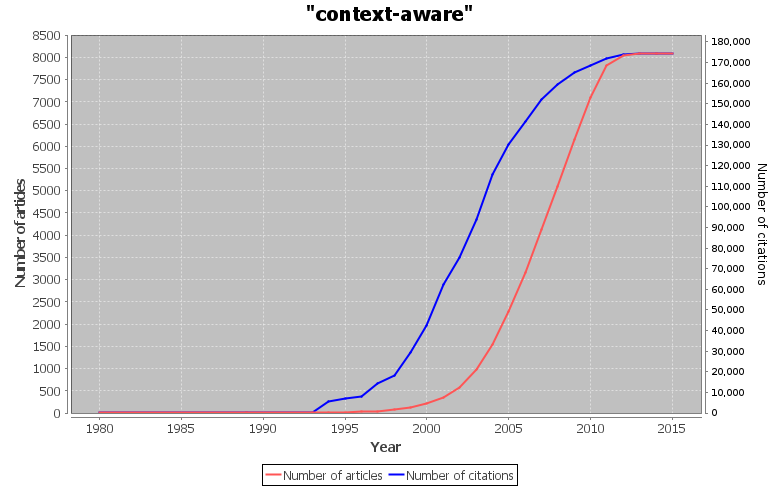
\includegraphics[width=\textwidth]{scholar-context-aware}
	\caption{Google Scholar and Microsoft Academic Search accumulated trending for ``context-aware'' query \cite{Rus:scholar-trends}.}
	\label{fig:scholar-context-aware}
\end{figure}

\begin{figure}
	\centering
	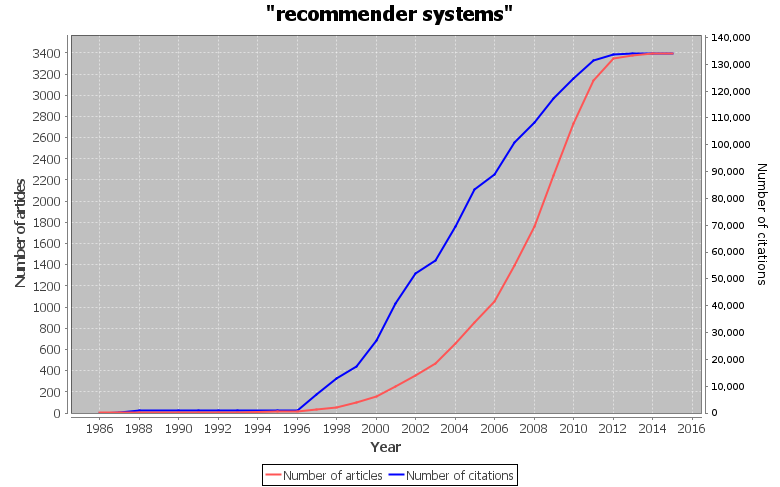
\includegraphics[width=\textwidth]{scholar-recommender-systems}
	\caption{Google Scholar and Microsoft Academic Search accumulated trending for ``recommender systems'' query \cite{Rus:scholar-trends}.}
	\label{fig:scholar-recommender-systems}
\end{figure}

\section{Context-aware systems}
\label{sec:context-aware}

The term, context-awareness, refers to the ability of the system to sense/be aware of its environment. This term mainly applies to mobile systems which are more likely to have their surroundings changed frequently. It is in a way similar to location awareness but expands beyond just location. Various researchers identify different elements of the context, e.g.:

\begin{itemize}
	\item user, role, identity \cite{Dey:context} \cite{Kaltz:context},
	\item process, task \cite{Kaltz:context},
	\item location \cite{Dey:context} \cite{Kaltz:context},
	\item time \cite{Dey:context} \cite{Kaltz:context},
	\item device \cite{Kaltz:context},
	\item activity \cite{Dey:context},
	\item nearby people and devices \cite{Rosslin:context},
	\item lighting and noise level \cite{Rosslin:context},
	\item network availability \cite{Rosslin:context},
	\item even the social situation (relations between the user and their peers nearby) \cite{Rosslin:context}.
\end{itemize}

By keeping track of this variables over the period of time, a system that would be classified as a context-aware one, could infer things that would be useful to the user. These might include turning on appropriate application on a mobile device when a certain set of conditions is met etc.

Context awareness is also an important concept in so called ubiquitous computing or just \emph{ubicomp}. To the regular user, ubicomp---also called pervasive computing and, more recently and commercially, Internet of Things---appears as if the computing processes were happening literally anywhere between a large network of distributed devices. These small, inexpensive devices equipped with various sensors share information among themselves as well as with services run by manufacturers, in order to provide the end user with some greater value.

Some exemplary use cases for a ubiquitous system might include:

\begin{itemize}
	\item ``domestic ubiquitous computing environment might interconnect lighting and environmental controls with personal biometric monitors woven into clothing so that illumination and heating conditions in a room might be modulated, continuously and imperceptibly'' \cite{wiki:ubiquitous},
	\item ``refrigerators «aware» of their suitably tagged contents, able to both plan a variety of menus from the food actually on hand, and warn users of stale or spoiled food'' \cite{wiki:ubiquitous}.
\end{itemize}

Thus, it is safe to say that ubiquitous computing would not be able to function without context-awareness.

An interesting research that is taking place in recent years, and is definitely worth taking a closer look at, concerns data gathered by the AWARE Framework.

AWARE Framework is an application and a library with a main purpose of gathering mobile context information. Analyzed sensors include: accelerometer, barometer, battery, running applications, Bluetooth, communication activities, gravity, gyroscope, locations, the level of light, network connectivity, temperature and many more. \cite{aware}

The collected data is sent to a pre-configured web service running a SQL data base in the back-end, where it can afterwards be analyzed by researchers. Furthermore it provides non-academic developers to enhance User Experience of their applications. By using the context information, they are able to plan notification/interruption moments more sanely. \cite{aware}

Choosing which elements of context are relevant for a given case is quite demanding, as there are many points to take into consideration. As AWARE developers put it, ``Capturing context is challenging. In fact, context is produced anytime, anywhere, by everything and anyone: it is extremely volatile and subjective.'' \cite{aware} One also has to think of such a mundane question as\ldots battery life of the mobile device.

\vspace{4cm}
\todo{Cite something by S. Bobek}

\clearpage

\section{Recommender systems}

According to \cite{Ricci:recommenders}, recommender systems are computer systems that may be used to predict ratings their users would give to certain items. In other words, these systems are able to predict (obviously, to some degree of correctness) which items would be most likely to be chosen by the user to interact with. In recent years, the solutions grew in popularity so much, that it is hard to imagine our digital lives without them. Classes of recommended items include:

\begin{itemize}
	\item entertainment: books, music, news, movies,
	\item restaurants, concerts, museums, places in general,
	\item interestingly, search queries (when we get intelligent suggestions after starting to type our queries into Google's search engine),
	\item help with (semi-)manual classification: hash-tags, social tags, question tags on question-oriented sites like Quora or StackExchange etc.,
	\item contacts: new friends on Facebook (the ``Friends \& People You May Know'' feature), new people to follow on Twitter (the ``Who To Follow'' or ``WTF'' feature) and also people one might be interested in on online dating services,
	\item financial services, life insurance policies. \cite{Felfernig:recommenders}
\end{itemize}

Recommender systems can be divided into three types.

\begin{enumerate}
	\item Collaborative filtering.
	\item Content-based filtering.
	\item Any mix of the two above (the so-called \emph{hybrid recommender systems}).
\end{enumerate}

\subsection{Collaborative filtering}

Collaborative filtering method works by looking at user's past behaviors, comparing them to other users of the system, finding most similar users and recommending items based on their decisions in the past. This model has several drawbacks (which, again, depend on the point of view):

\begin{itemize}
	\item a rather large amount of data is required for the system to provide valuable insight (the \emph{cold start} problem),
	\item at the same time care must be taken to make the system scalable; often, these systems face millions and millions of users and items,
	\item sparsity and scarcity of data (user explicit or implicit ratings) --- again, as there are millions of items, it is often the case that only some of the items are rated and theres not enough data to make necessary connections,
	\item all current realizations assume that users agreeing in the past will agree in the future (future understood as the recommendations to be made), which might not always be true.
\end{itemize}

The sparsity problem can be solved by inventing better methods of obtaining user ratings. These ratings can be generally classified 

While explicitness of asking a user to rate a movie is understandable---after all few people would complain, as it is obvious that the movie recommending system has to learn our likes and dislikes to build the proper model of our brains (and going through the movies we watched again and rating them is fun, too!)---when we start getting into e-commerce areas, it stops being justified right away.

This phenomenon might be explained psychologically. When interacting with a movie recommender, the person wants to get some great new recommendations, they are willing to pay for them with their ratings. On the other hand, the commercial recommender is seen as one wanting to take advantage of the user, make them buy some more items and in turn make even more money. This negative image can only be overturned by the system recommending just the right items (from the user's perspective).

One of the most popular collaborative filtering algorithms is the \emph{item--to--item} one, originally popularized by Amazon (the ``people \todo{Mention explainability?}who buy A buy also B'' feature), used also by Facebook and LinkedIn and Twitter for new friends and groups suggestions, and Last.fm for new music recommendations.

\subsection{Content-based filtering}

The second approach to recommending is content-based filtering. These methods are in turn based on comparing distinctive features of the recommended items to the user's preferences, instead of on what other people (similar to the user) think of them.
\chapter{Rule-based systems, HeaRTDroid}
\label{cha:rules}

\chapter{Micro-location}
\label{cha:microlocation}

% Motivation

The primary motivation for providing an ultimate solution to the micro-location problem is enabling a new wave of mobile---possibly artificially intelligent---applications. Possible uses of micro-location are unimaginably limitless (by analogy, it suffices to browse through endless lists of mobile applications for the ``GPS'' query in any application store). Below, there are some of the most quick and straightforward ideas.

\begin{itemize}
	\item Museums were the main use case when this project came to life, as they are the most obvious one. One can imagine walking through Louvre with their own smartphone describing all exhibits \emph{interactively}! Almost like walking with one's own rented guide. And with the advances in artificial intellect, this experience might start to become more and more like it.
	
	\item Big shopping centers and malls could benefit greatly from micro-location capabilities. Users (customers) would no longer got lost. (Or, arguably, is it to the center owners' benefit that they got lost?) Especially so, if micro-location data was used with customer profiling, machine-learning what they might want to buy and why.
	
	\item Large building of some public (to a certain extent) services, like government buildings, campuses, big office buildings, enormous hospitals\ldots While their employees may know arrangements and purposes perfectly, it's not that clear to customers, citizens, students, people who visit these buildings for the first time in their lives.
	
	\item Another category of public space is various venues related to transportation of---mainly---people. Airport, train stations buried deep underground might overwhelm some, especially if there are only five more minutes left to get on one's next line. Precise navigation accompanying the user can be imagined to be at least a blessing.

	\item We need not forget businesses now using custom micro-location technology to aid their workers (or machines working for them) in locating themselves in the vast spaces occupied by warehouses, workshops, storage facilities or even mines with corridors outstretching through the depths of Earth. These businesses could just use their workers' smartphones, they use daily. It's worth noting, that custom solutions are often more expensive; and probably always \emph{more} expensive, when the alternative is used by 2 billion other devices.
\end{itemize}

If correctly working micro-location was widely available, there would probably emerge a place for some centralized service holding most---if not all---of the indoor navigational maps, like Google Maps does for GPS and outdoor data, mapping the whole world. Or, more likely, an application able to use openly distributed data about public space buildings, but at the same time with an option to plug in---possibly with some kind of authentication---into non-public maps. That could be of use when confidential data becomes involved (plans of classified government buildings, business secrets etc.).

Undeniably, in recent years, a new truth has become more and more prominent and at this point, it would be really dishonest not to mention importance of User Experience. It's even more visible in the field of localizing devices. GPS-based outdoor navigation annoys the user heavily, when it misleads them. In addition to the possibility of misleading, the proposed method is based on \emph{mediation} (\cref{sec:mediation})---indirectly asking the user where they are---something, that already will annoy them to some degree. More about the not-so-good User Experience of this particular method can be found in \cref{sec:user-experience}.

Below, both more and less promising solutions for this problem already existing today are described. Some of them are used in the micro-location method proposed in this paper; in these cases the relation is discussed briefly. More details can be found in \cref{sec:physics-module}.

\section{Overview of existing solutions for micro-location}
\label{sec:existing-uloc}

It is worth noting, that most methods below incorporating electromagnetic signals use the law of inverse square which says that a quantity or---in this case---intensity of some field is inversely proportional to the square of the distance from the source.

\begin{equation}
	\label{eq:inverse-sq}
	I \propto \frac{1}{r^2}
\end{equation}

In this field---pun intended---also called RSSI (or Received Signal Strength Indication) \cite{Gough:RSSI}.

Some of the other methods make extensive use of the triangulation technique known in its current form since the 17th century. In triangulation, when both two angles of the triangle are known and the distance between their vertices (length of the side), the law of sines may be used to calculate the distance from the side to the third vertex (the height of the triangle). \Cref{fig:triangulation} illustrates this well. In micro-location use cases, the vertices near $\alpha$ and $\beta$ angles are simply sensors of some electromagnetic signals.

\begin{figure}[h]
	\centering
	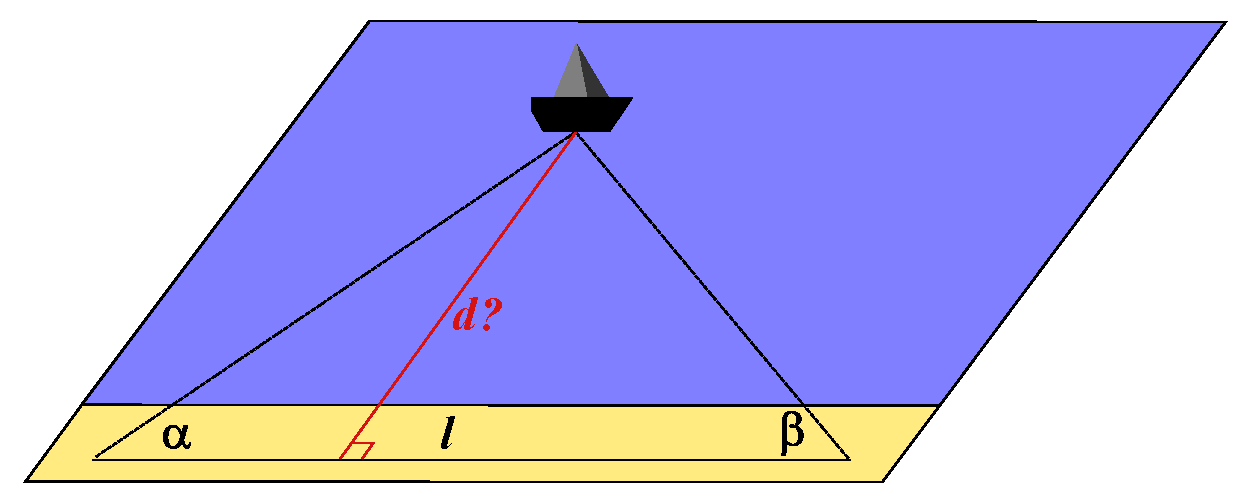
\includegraphics[width=0.67\textwidth]{triangulation}
	\caption{Triangulation. By knowing $\alpha$, $\beta$ and $l$ beforehand, the distance $d$ from the ``ship'' to the side of length $l$ can be calculated using the sine formula (or law of sines) \cite{wiki:triangulation}.}
	\label{fig:triangulation}
\end{figure}

\begin{description}
	\item[Magnetic positioning] is a technique that uses data from smartphone's magnetic sensor, the compass. Most buildings nowadays use reinforced concrete (concrete with steel bars as a skeleton, see \cref{fig:reinforced-concrete}). These bars affect Earth's magnetic field in a unique way \cite{Haverinen:magnetic}. Crowd sourcing may be used to map a building and, later, these maps may be used to locate a device indoors. This technique gives accuracy of 1--2 meters with confidence level of 90\%. However, it is not really that perfect, as the measurement is heavily impacted by moving metal objects inside the building such as elevators, drawer cabinets etc.
	
	\begin{figure}[h]
		\centering
		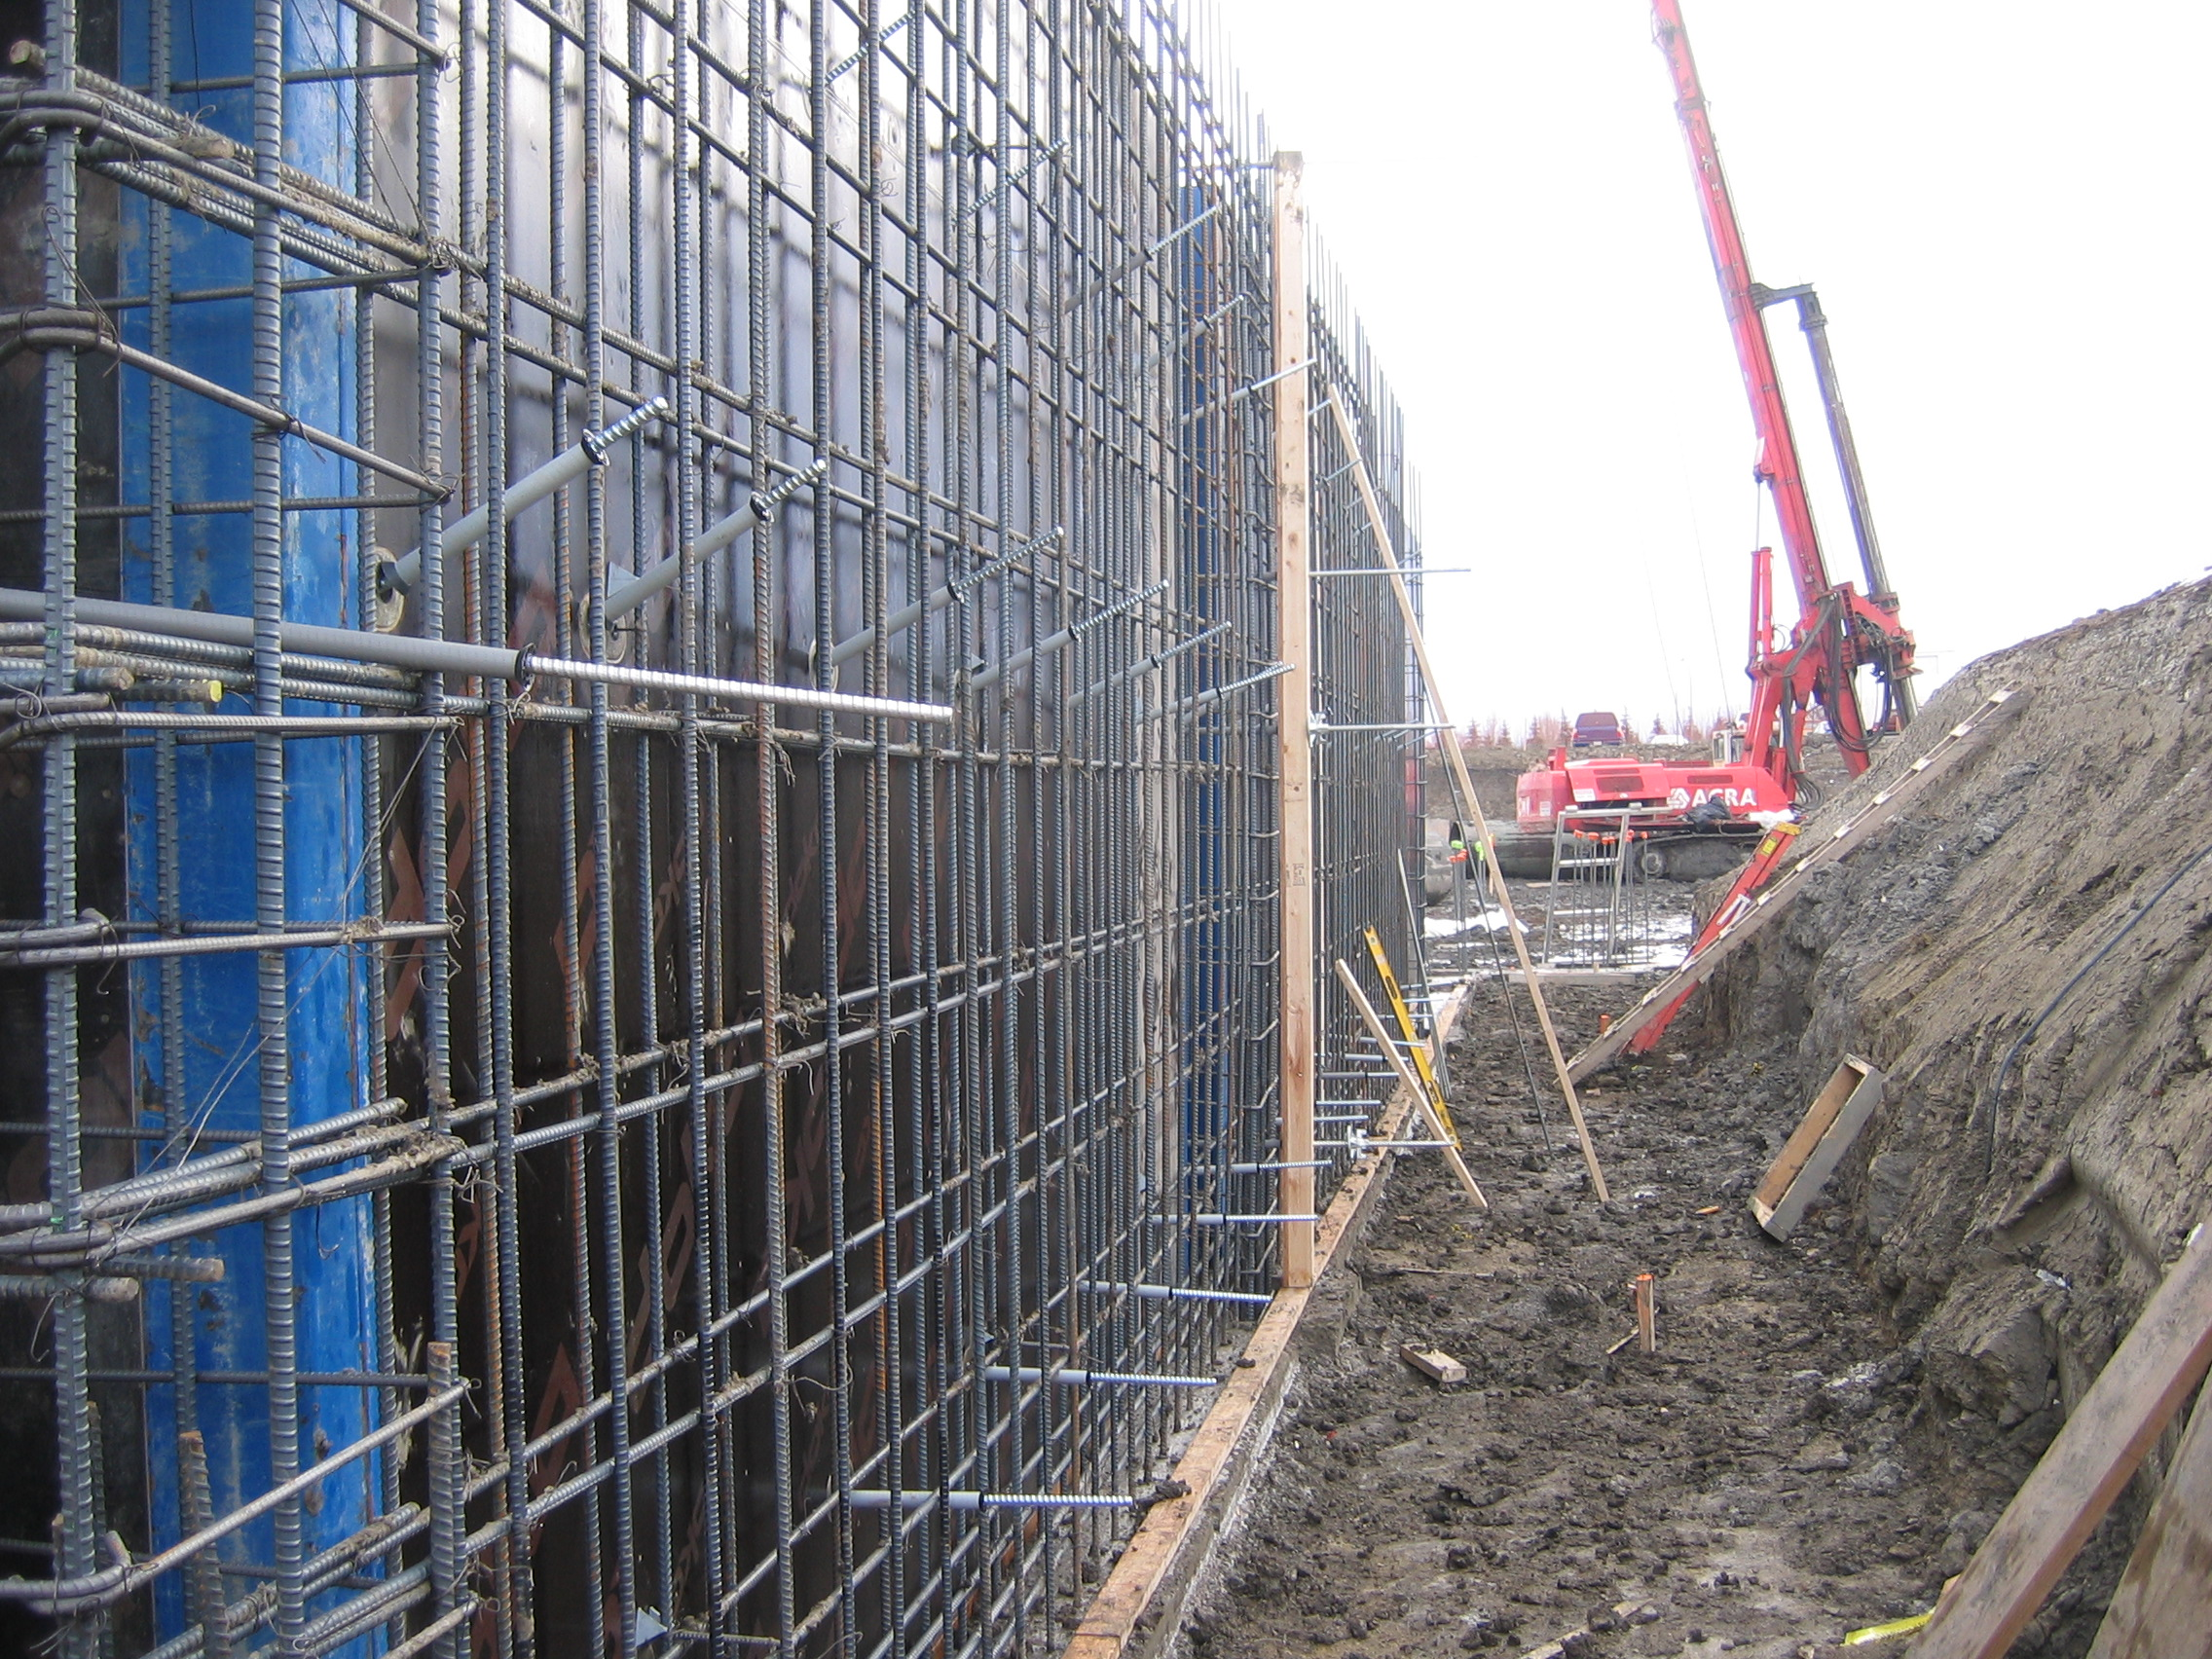
\includegraphics[width=0.67\textwidth]{reinforced-concrete}
		\caption{Steel bar construction prepared for turning into reinforced concrete (still, before pouring the concrete) \cite{penco:concrete}.}
		\label{fig:reinforced-concrete}
	\end{figure}
	
	\item[Inertial measurements] is a pedestrian \emph{dead reckoning} technique and as such is a subject to cumulative errors (among others). When used in a smartphone, built-in sensors---accelerometers in all three axes---provide data from which distinct human steps in time and space can be inferred (see \cref{fig:inertial-measurements}). Later, these steps are overlaid with maps that had to be previously created and user's location is guessed. Even the smallest error made early in this dead reckoning process will manifest itself in every following result, as position $i+1$ is position $i$ with data about $i$-th step added to it. Accelerometers are also pretty noticeable when it comes to battery performance. A lot more energy is being consumed when these sensors are on. Having all these three disadvantages in mind---cumulative errors, battery life and inability to automatically map a previously unknown environment---this is one of the chosen techniques used in physics-based module that provides alternatives for mediation method described in this work (see more about the module in \cref{sec:physics-module}).
	
	\begin{figure}[h]
		\centering
		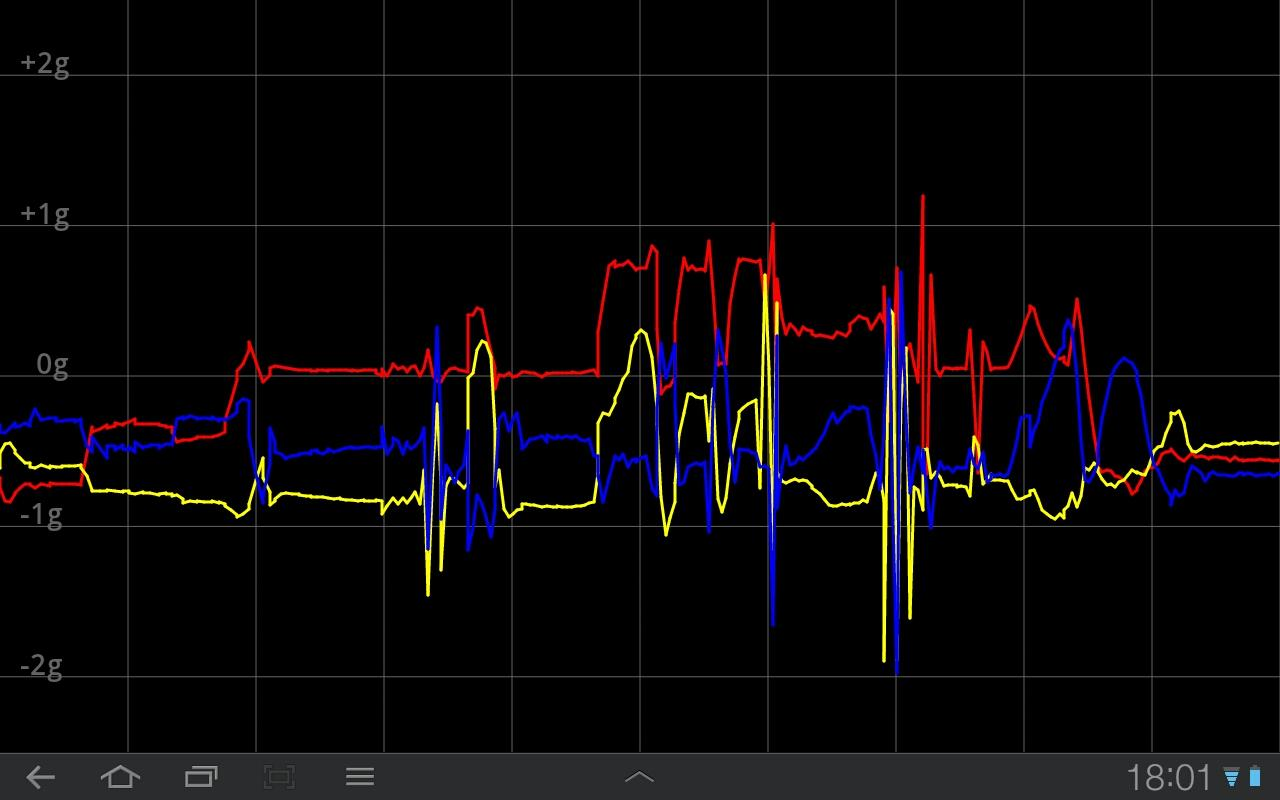
\includegraphics[width=0.67\textwidth]{inertial-measurements}
		\caption{Screenshot of an Android application plotting sensory data from accelerometers in all three axes in real time \cite{google-play:accelerometer}. Some steps can even be seen with the naked eye (the steep fragments).}
		\label{fig:inertial-measurements}
	\end{figure}
	
	\item[Wi-Fi-based positioning] uses information about signal strengths of all visible Wi-Fi networks at a given moment (see \cref{fig:wifi-positioning}). From these strengths, using the Received Signal Strength Indication, we can infer distances to all visible access points. Positions of these are known from a previously prepared map. Using these positions and distances, user's location may be easily obtained. Again, it is possible for signal fluctuation to influence the correctness of this method. One notable realization of this method is ``Anyplace'' from researchers at the University of Cyprus \cite{Anyplace}.
	
	\begin{figure}[h]
		\centering
		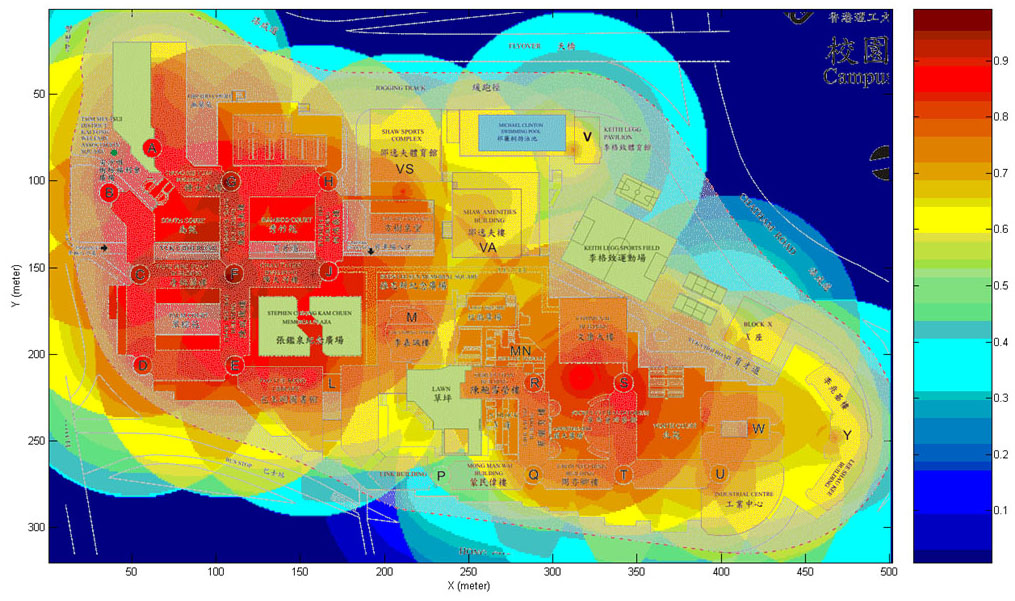
\includegraphics[width=0.67\textwidth]{wifi-positioning}
		\caption{A heat map of Wi-Fi signal strengths at the Hong Kong Polytechnic University \cite{hk:wifi-positioning}.}
		\label{fig:wifi-positioning}
	\end{figure}
	
	\item[iBeacons (via Bluetooth)] are small devices using Bluetooth LE (Low Energy) technology standardized by Apple in 2013. These devices constantly broadcast their unique identifiers to all nearby devices. UUIDs are simply 128-bit numbers usually notated in hexadecimal format, e.g. \texttt{e16d9b56-4d95-48f6-959b-4c8bf701bc6f}. Because of using LE, usually only devices in the same room as the transmitting beacon can receive the signal and by that know what room they're in. Obviously, one has to previously map UUIDs to rooms. Also, not all smartphones currently in use support Low Energy variant of Bluetooth, and thus not all are compatible. Another advantage of using Low Energy variant of Bluetooth  This technique is also used as one of the sources in the physics module (\cref{sec:physics-module}).
	
	\item[RFID] is an acronym for radio-frequency identification. This method is similar in its concept to iBeacons. Small chips with unique identifiers are placed in the room (see \cref{fig:rfid} for some examples of such chips). RFID reader knows the mapping between chips' IDs and rooms/positions. When an ID is read, its matching room is chosen as the user's current location. One big disqualifying disadvantage is that today mobile phones are not RFID readers.
	
	\begin{figure}[h]
		\centering
		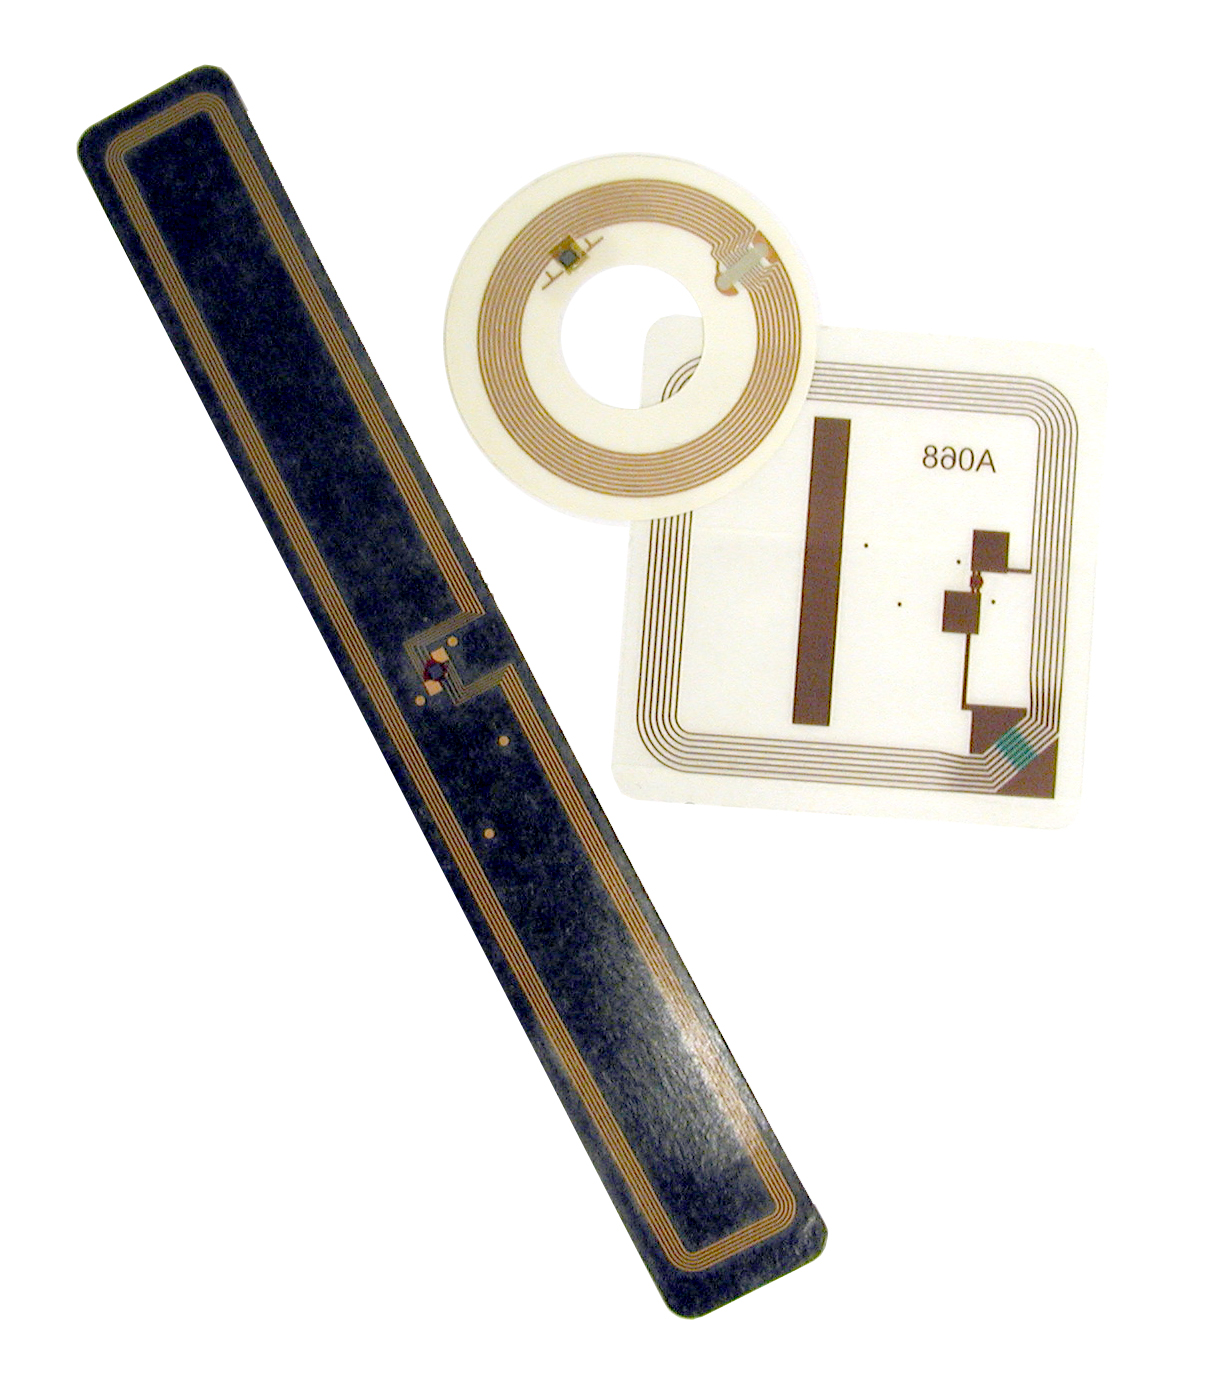
\includegraphics[width=0.5\textwidth]{rfid}
		\caption{Examples of RFID chips used for tagging items and locations \cite{wiki:rfid}.}
		\label{fig:rfid}
	\end{figure}
	
	\item[Grid concepts] revert the receiver and transmitter roles. A device being micro-located broadcasts its identification information, usually by using RFID technology. A large number of receivers are arranged in a grid pattern over an area under observation. Low energy of the signal guarantees that only the receivers closest to the transmitting chip will get its identification. Because of these considerations this method is not readily available for today mobile phones.
	
	\item[Angle of arrival] methods usually need to operate on an array of antennas. Each sensor in the array gets the signal at slightly different time (see \cref{fig:cross-corr-pulse} for a method of calculating this difference). From this time difference of arrival---or TDOA---for the whole array, the angle of arrival can be calculated. Other solutions use highly directional receivers arranged in a circular pattern. A receiver that gets the signal, determines the angle. After having the angle measured for at least 2 distinct transmitters, in the next step, the angles are used during triangulation (\cref{fig:triangulation}) which, in the end, provides array's position.
	
	\begin{figure}[h]
		\centering
		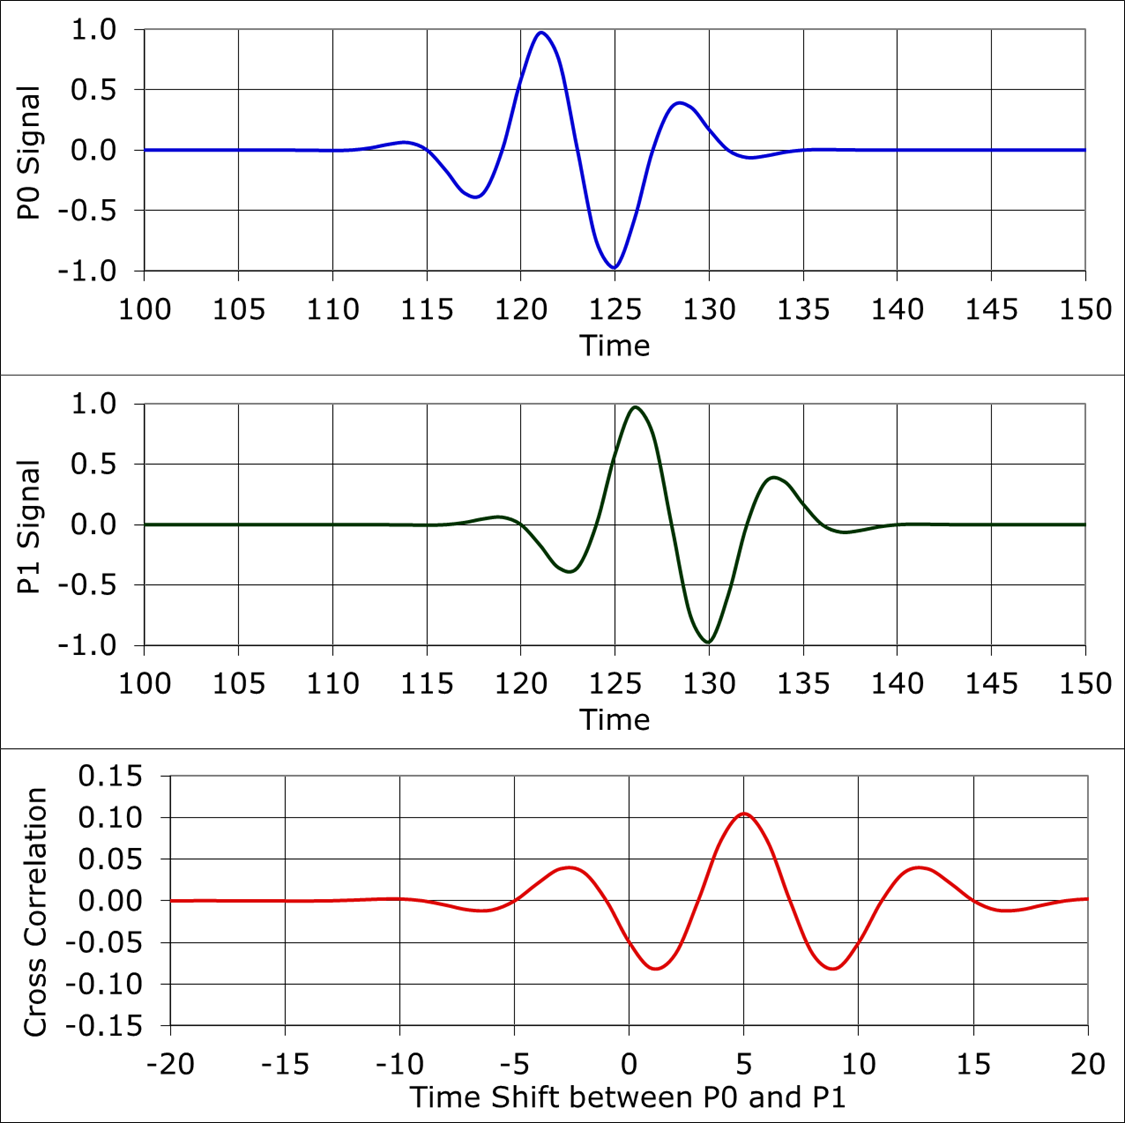
\includegraphics[width=0.67\textwidth]{cross-corr-pulse}
		\caption{Cross correlation between two upper signals shown as the third signal \cite{wiki:cross-corr-pulse}. Maximum in $t=5$ suggests that the signals are shifted by $5$ time units.}
		\label{fig:cross-corr-pulse}
	\end{figure}
	
	\item[Time of arrival] method is slightly similar to \emph{angle} of arrival. When time the signal took to get from a transmitter to a receiver is known, and so is its propagation speed, the traveled distance can be calculated straightforwardly. Transmitted signal has to encode some kind of a time marker, marking the time of sending. The main instantly visible problem here is\ldots extremely accurate time synchronization needed between the both parties. This technique is used in GPS, which is the reason for it being able to be used as a time source.
	
	\item[Ultra-wideband] (also called UWB) is radio transmission method that uses a wide part of the radio frequency spectrum and extremely low energy to transmit large amounts of data over very short distances \cite{ultra-wideband}. These short distances are of interest here, as we don't want to receive signals from other rooms. Unfortunately, modern smartphones are not compatible with this radio technology.
	
	\item[Infrared] communication requires that receivers and transmitters ``see'' each other. Thanks to that, locating based on infrared light would be confined to a single room, a desirable trait. Infrared sensors used to be popular in mobile phones, but this popularity decreased dramatically with the advent of smartphones. Nowadays, it's usable only in custom deployments.
	
	\item[Visible light communication] method is similar in its concept to the infrared-based one. One major difference is that all smartphones have visible light sensors built in, the camera. Zhang and Kavehrad propose a method for indoor localization system based on visible light LEDs \cite{Zhang:visible-light}. Its computer model is able to localize a device in two dimensions with accuracy of centimeters for a reasonably sized room. Along with localization using local warps of Earth's magnetic field, this method is one of the most promising ones. One blatant downside would be the need to lay out the diodes in all rooms being observed, while magnetic positioning works almost out-of-the-box.
	
	\item[Ultrasound] positioning offer much greater accuracy due to the fact that sound travels through air at a \emph{lot} slower speeds than light or other electromagnetic signals. The method works---similarly to RFID positioning---by having simple tags attached to to-be-located objects transmit ultrasound identifying information. Again, such a method cannot be used with currently marketed mobile devices, as these lack capabilities of projecting ultrasonic---in this case---signals with their unique IDs.
	
	\item[QR codes] (abbreviation for Quick Response codes) is a trade name for a particular type of two-dimensional barcode (see \cref{fig:qr-code} for an example of such a code). This method of micro-location is \emph{similarly burdensome and awkward} for the user as the method proposed in this paper (more about bad User Experience in \cref{sec:user-experience}). It works by---first---having these graphical codes laid out in the observed building. Each of them is encoding either a unique identifier of the exact spot it's placed at or even just information about that location directly. Next, the user has to scan a code---take a picture, basically, and then wait for its processing---if they want to learn where exactly this code is physically placed (i.e. just read off information encoded in the QR). Downsides: a lot of preparation needed on the side of the building's management and a lot of awkward hassle for the user. It's worth noting that there exists an Internet movement among software developers aimed at discouraging QR code use to the point of total elimination from public space \cite{should-i-use-qr}.
	
	\begin{figure}
		\centering
		
\includegraphics{qr-code}
		\caption{Sample QR-code, version 10 \cite{wiki:qr-code}.}
		\label{fig:qr-code}
	\end{figure}
	
	\item[NFC] is an abbreviation for Near Field Communication. NFC allows enabled devices to establish a radio connection over a very close range (less than 10 cm). This necessary closeness can be used to locate a device with confidence, as the user has to almost touch a tag with their device (so they have to be near it), to read it. At the same time this requirement renders this method highly impractical and burdensome for the user. The NFC technology is only built into new smartphones by Apple and most premium Android phones, and because of that it is not compatible with most devices currently in use. These points don't stop some researchers from publishing a paper about their proposed framework for such a micro-location method \cite{nfc-ulocation}. As a tidbit, this is also the technology used in contactless payments using credit and debit cards.
	
\end{description}

\section{Mediation. The proposed method}
\label{sec:mediation}

\todo[inline]{Motivation for using semantic maps}

\chapter{Results}
\label{cha:results}

\section{Mediation. The proposed method}
\label{sec:mediation}

\section{Physics-based module for providing alternatives}
\label{sec:physics-module}

\todo[inline]{something about inertial measurements}

\todo{something about beacons} Arguably, this is somewhat of a misuse of the beacons technology. Manufacturers generally speak of only \emph{three} recognizable levels of ``interaction'' with the beacon (based on signal strength): \begin{itemize}
 	\item receiver being in very close proximity to the transmitter,
 	\item receiver being in the same room,
 	\item no interaction at all.
 \end{itemize}
 
The idea for using beacons in the module is to make an assessment about distances to nearby transmitters based on signal strength and law of inverse squares (see \cref{eq:inverse-sq}). Wojnicki et al. claim that this works; however, \emph{only under laboratory conditions}. \todo{cite Wojnicki} As iBeacons use extremely low energy to transmit the signal, even a person walking across the room while taking the measurement can influence it so negatively, that any information inferred about the signal's distance is almost worthless.

\section{Architecture of the proposed solution}

\todo[inline]{describe architecture etc.}

\section{User Experience}
\label{sec:user-experience}

\chapter{Examples, evaluation}
\label{cha:evaluation}

\section{Case 1: AGH UST building}

\section{Case 2: Main Square, Kraków}

\chapter{Summary}
\label{cha:summary}

As the project is able to correctly infer user location, given correct answers to the questions generated using data encoded in OpenGIS maps of some area, the design criteria were met. There are, however, some issues that need to be mentioned. Also, suggestions for potential future work are presented.

One of the most glaring deficiency of this solution in its current state is lack of the concept of transparency. This is especially visible in the second evaluated case (\cref{sec:case-cracow-square}). While that case was clearly about location outdoors, and it was presented just to showcase that mediation is limited not only to indoor micro-location, it is still possible to encounter transparency indoors. Some objects might still be visible while really being located outside of a given alternative. Examples might include indoor windows, . User, when asked if they see that object, would answer positively, ruining the inference. It is here that the relations planned (see \cref{sec:ontology}) and the concept of closeness might come into play.

Also, if some kind of relations were implemented, it could be possible for the question generator to choose more \emph{interesting} questions from human perspective. E.g. a chair standing \emph{on} a desk is certainly interesting, rare, unusual for a human. However, encoding such human-centered (non-)weirdness might turn out too difficult to accomplish efficiently.

The current solution works under the assumption that users won't lie. When there are several alternative locations possible, the ``happy path'' flow of narrowing down to only one location is linear and there is no possible way for the user to introduce any contradiction. Thus, no need for detection of contradictions. However, when the user decides they have made a mistake, the can take a step back and re-answer the previous question (or second but last etc.).

Use of dead-reckoning based on pedometer implemented in the physics module may be disputable, as it will simply not work correctly, when the user is not moving on foot. However, that decision is not in the scope of this work.

From a technical standpoint, there are also several issues that might be addressed in the future. Two most obvious optimizations come to mind. Matching costs (from the configuration file) to particular objects could be improved. Currently the whole maps provided by the user are read into memory before processing. It might be possible to stream-read them as needed. However, both of these optimizations were not necessary performance-wise for friction-less experience with the evaluated use cases. Also, the map parser could be enabled to read other, more up-to-date formats, like GeoJSON\footnote{\url{https://web.archive.org/web/20150801152712/http://geojson.org/}, visited on 08/01/2015.}.

Finally, the User Experience needs to be brought up. Nowadays, when creating a dedicated technical solution, its UX has to be thought over thoroughly, as---simply put---users are spoiled by constant innovations in this area.

The solution proposed in this paper, makes the user answer several questions about their surroundings, before being able to tell where they are. It is quite counterintuitive, as the expectation for a \emph{location system} is that \emph{the system} is---almost magically---able to answer the question of where the user is (cf. GPS). There seems to be no way to make that experience tolerable---if not pleasurable---for the user, while keeping the design objectives unchanged. This claim is confirmed by 30+ people I talked to about a possible mobile application implementing the method. Vast majority of them laughed at the idea, saying they would instantly remove such an application from their device, a reaction of little motivational value.

The above seems to cause the method to be unusable as a business solution. Perhaps it would turn out acceptable in an informal setting---e.g. as a game of some sort---or maybe even in half-formal environment like a museum, as a potentially helpful yet awkward and burdensome electronic/software guide.

To sum up, I would risk a claim that some new, technology is needed, dedicated solely to micro-location. All existing smartphones need to be scrapped as soon as possible. As costly, as it might seem, when looking at the available solutions (\cref{sec:existing-uloc}) and overwhelming inconvenience of this method (User Experience), this is the only real option. And by ``real'' I mean something that might turn out usable to the ordinary person in not-so-distant future.

It's also worth mentioning, that the mediation in this case has little sense, as iBeacons themselves give \emph{exactly} the information we were after: ``which room am I in?'' Answering that question was the main design objective for the iBeacon technology (and this project, too). Thus, instead of having several beacons in one room (317 from the AGH-UST example, \cref{sec:case-agh}), one beacon could be placed in each room under observation. Nevertheless, this work can be thought of as a research exercise.


\cleardoublepage
%\bibliographystyle{alpha}
%\bibliography{bibliography}

\printbibliography

\appendix
\chapter{Licensing, source code}
\label{cha:source}

\todo{use Apache2 and put it on GitHub like I did with my \href{https://github.com/michalrus/agh-mindmap}{BSc}}


\end{document}
